%====================
\chapter{Les graphes}
%====================

\begin{center}
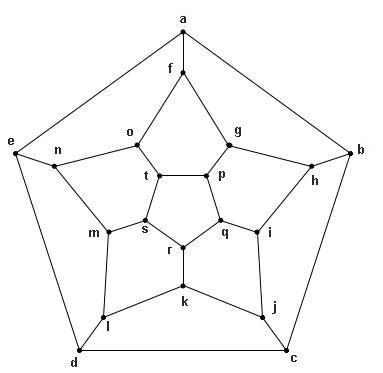
\includegraphics[width=4.092cm,height=3.999cm]{image/a2012Logique2eme-img041.jpg}
\end{center}
	

%================
\section{Utilité}
%================

	La théorie des graphes permet de répondre à différents 
	problèmes se formulant en termes d'\textbf{objets} et de
	\textbf{liens} entre ceux-ci. De nombreux problèmes relatifs 
	à l'étude des réseaux peuvent être résolus grâce à la
	théorie des graphes, que ce soit des problèmes de voyage 
	(réseaux aériens, routiers, ferroviaires) ou des problèmes de
	communication entre personnes (réseaux téléphoniques) 
	ou entre ordinateurs (réseaux informatiques, internet{\dots})

	Un problème classique de la théorie des graphes, et qui a 
	prouvé toute son utilité depuis l'invention du GPS, est la
	détermination du chemin le plus rapide (ou le plus court 
	ou encore le moins coûteux) entre deux localisations
	géographiques. Pour résoudre ce type de problème, il faut 
	connaitre les différents relais ou points de passage (objets)
	et savoir lesquels sont reliés entre eux par des routes 
	(les liens), ainsi que des informations supplémentaires sur ces
	liens (distance, type de route, etc.).

	Un autre pilier de la théorie des graphes est l'étude de 
	l'ordonnancement des tâches. Quelles sont les contraintes
	conditionnant l'avancement d'un projet ? Quelle tâche doit 
	être finie avant que telle autre ne commence ? Comment tenir
	compte des tâches concurrentes ?

	D'autres domaines peuvent également être abordés~:

	\begin{itemize}
		\item {
			analyse d'un programme, d'un algorithme}
		\item {
			élaboration de cartes géographiques}
		\item {
			représentation de relations entre individus (familiales, professionnelles{\dots})}
		\item {
			représentation d'automates d'états finis, de tables de décisions{\dots}}
	\end{itemize}
	
	Le but de cette partie du cours n'est pas d'aborder jusque 
	dans les moindres détails la théorie des graphes. Celle-ci et
	ses développements sont d'une telle richesse qu'ils font 
	l'objet de nombreux ouvrages spécialisés. Nous nous limiterons
	à un aperçu synthétisé permettant de situer les problèmes et de 
	servir de tremplin à une étude personnelle plus approfondie.

%=====================
\section{Terminologie}
%=====================

	N.B.~Les graphes vous sont déjà familiers, puisqu'ils 
	ont déjà été étudiés au cours de mathématique de
	1\textsuperscript{ère} année. Nous rappelons brièvement 
	ici les principales définitions, et renvoyons le lecteur au
	syllabus de mathématique de 1\textsuperscript{ère} 
	pour plus de précision.

	\subsection{Définition}
	%======================

		Un \textbf{graphe} est un modèle mathématique représentant 
		les liens existant entre différents objets de même type,
		appelés \textbf{n{\oe}uds} ou \textbf{sommets}. Les liens 
		sont appelés \textbf{arcs} ou \textbf{arêtes}, selon que le
		graphe est orienté ou non. On peut donc voir un graphe comme 
		l'association de l'ensemble $S$ de ses n{\oe}uds et de
		l'ensemble $A$ de ses arêtes~:

		\begin{center}
			$G = (S, A)$
		\end{center}


		On représente schématiquement un graphe par un ensemble de 
		points reliés entre eux par des traits ou des lignes
		représentant ces liens.

	\subsection{Types de graphes}
	%=============================
	
		\subsubsection{Graphe orienté}
		%=============================
		
			Un graphe est \textbf{orienté} lorsque ses n{\oe}uds 
			sont reliés par des \textbf{arcs}. Un arc est un \textbf{couple}
			$(u, v)$ de n{\oe}uds, où $u$ est l'\textbf{origine} du couple 
			(ou encore le \textit{prédécesseur}, le	\textit{départ} ou 
			l'\textit{extrémité initiale}) et $v$ l'\textbf{extrémité} 
			(ou encore le \textit{successeur}, l'\textit{arrivée} ou 
			l'\textit{extrémité terminale}). On dira de cet arc qu'il 
			\textit{part} du n{\oe}ud $u$ et qu'il \textit{arrive} au 
			n{\oe}ud $v$. Dans la représentation schématique d'un graphe 
			orienté, on représente habituellement les arcs par des flèches 
			qui traduisent le sens de la relation entre deux n{\oe}uds.

			\textbf{Exemple~:} G = (S, A) avec S = \{A, B, C, D, E\} et 
			A = \{(A, D), (A, E), (B, A), (B, E), (C, A), (C, E), (D, B), (D, C),
			(E, D)\}

			\begin{center}
			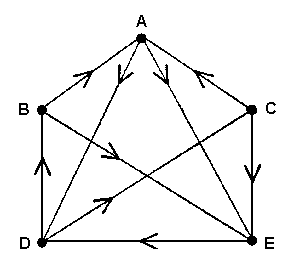
\includegraphics[width=5.159cm,height=4.598cm]{image/a2012Logique2eme-img042.png}
			\end{center}
			
			Un graphe orienté peut aussi contenir des boucles~: 
			une \textbf{boucle} est un arc dont l'origine et l'extrémité sont
			identiques, elle part et arrive au même n{\oe}ud.

			Un graphe orienté est dit \textbf{symétrique} si l'existence 
			d'un arc allant de $u$ vers $v$ implique l'existence d'un arc 
			«~réciproque~» de $v$ vers $u$ (avec $u \neq v$).
			

		\subsubsection{Graphe non orienté}
		%=================================
			
			Dans un graphe \textbf{non orienté}, les n{\oe}uds sont 
			reliés par des \textbf{arêtes}. Une arête est une \textbf{paire}
			$\{u, v\}$ de n{\oe}uds, c'est-à-dire un ensemble non ordonné 
			de deux n{\oe}uds (pour rappel,
			$\{u, v\}$ = $\{v, u\}$)

			\textbf{Exemple~:} G = (S, A) avec S = \{A, B, C, D, E, F\} et 
			A = \{\{A, B\}, \{A, E\}, \{B, C\}, \{C, D\}, \{C, F\}, \{D, E\},
			\{D, F\}, \{E, F\}\}

			\begin{center}
			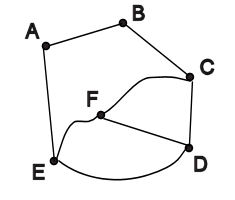
\includegraphics[width=4.284cm,height=3.657cm]{image/a2012Logique2eme-img043.jpg}
			\end{center}

			Remarquons qu'un graphe non orienté peut être représenté par un 
			graphe orienté~: il suffit de remplacer chaque arête
			reliant deux n{\oe}uds distincts par deux arcs orienté (ce qui donne 
			un graphe symétrique). L'inverse n'est évidemment pas vrai !

		\subsubsection{Multigraphe}
		%==========================
			
			Lorsqu'on admet que deux n{\oe}uds d'un graphe peuvent 
			être rejoints par plusieurs arcs ou arêtes, on parle de
			\textbf{multigraphe}. Ce type de graphe est par exemple 
			utilisé en chimie pour la représentation des molécules, un
			double lien représentant une liaison plus forte entre 
			les atomes d'une molécule.

			\begin{center}
			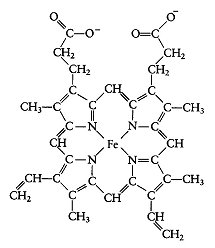
\includegraphics[width=5.172cm,height=5.974cm]{image/a2012Logique2eme-img044.jpg}
			\end{center}

		\subsubsection{Graphe pondéré}
		%=============================
			
			Lorsqu'on associe une valeur numérique à chaque arc ou 
			arête d'un graphe, on obtient un \textbf{graphe pondéré}.
			L'exemple le plus connu d'un tel graphe est la carte routière 
			sur laquelle on indique les distances le long des routes
			joignant deux points de repère. D'autres informations possibles 
			sont le temps, le coût, le poids{\dots}

			\begin{center}
			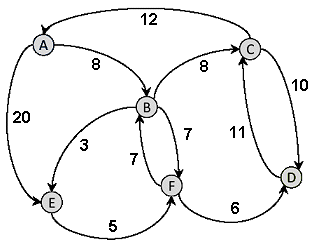
\includegraphics[width=9.038cm,height=7.091cm]{image/a2012Logique2eme-img045.png} 
			\end{center}
			
		\subsubsection{Graphe étiqueté}
		%==============================
		
			Un graphe est étiqueté lorsque ce sont des informations 
			de type texte qui sont attachées sur chaque arc ou arête (par
			exemple les numéros des routes sur une carte routière~: «~A19~» ou «~E40~»{\dots})


	\subsection{Adjacence, incidence et degré}
	%=========================================
		
		On dit que deux n{\oe}uds sont \textbf{adjacents} 
		(ou \textbf{voisins}) s'il existe un arc (pour les graphes orientés)
		ou une arête (pour les graphes non orientés) reliant ces n{\oe}uds. 
		L'adjacence s'applique aussi aux liens~: deux arcs (ou deux arêtes) 
		sont \textbf{adjacents} lorsqu'ils ont un n{\oe}ud en commun. 
		Par contre, la relation entre les n{\oe}uds et les liens s'exprime 
		en terme d'\textbf{incidence}~: on dit qu'un arc ou une arête est 
		\textbf{incident} à un n{\oe}ud.

		Un graphe non orienté dans lequel chaque n{\oe}ud est adjacent 
		à tous les autres n{\oe}uds est dit \textbf{complet}.
		Pour un graphe orienté, un graphe complet est tel qu'en 
		chaque n{\oe}ud partent des arcs vers tous les autres n{\oe}uds.

		Le degré d'un n{\oe}ud est le nombre d'arcs (ou d'arêtes) 
		incidents à ce n{\oe}ud. Dans le cas d'un graphe orienté, 
		on définit encore~:
		
		\begin{itemize}
			\item {
				le \textbf{degré entrant} d'un n{\oe}ud~: 
				c'est le nombre d'arcs qui arrivent en ce n{\oe}ud}
			\item {
				le \textbf{degré sortant} d'un n{\oe}ud~: 
				c'est le nombre d'arcs qui partent de ce n{\oe}ud}
		\end{itemize}
		
		Toujours dans le cas des graphes orientés, un \textbf{puits} 
		est un n{\oe}ud dont le degré sortant est nul~: arrivé dans
		un puits, on ne peut plus en sortir ! Inversement, une 
		\textbf{source} est un n{\oe}ud dont le degré entrant est nul.
		On peut donc partir d'une source, mais on ne peut plus 
		jamais y revenir ! Si les degrés entrant et sortant sont tous
		les deux nuls, on a alors un n{\oe}ud isolé.

		\textbf{Exemple~:} dans le graphe ci-dessous, 
		le n{\oe}ud 8 est de degré 3 ; son degré entrant est 2 
		et son degré sortant est 1.
		Les n{\oe}uds 1, 3 et 5 sont des sources, 
		et les n{\oe}uds 6 et 7 sont des puits.

		\begin{center}
		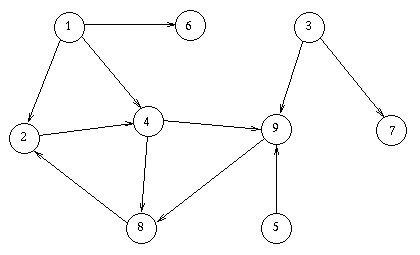
\includegraphics[width=7.527cm,height=4.56cm]{image/a2012Logique2eme-img046.jpg}
		\end{center}
		
		\textbf{Remarque~:} une boucle compte pour deux dans le calcul du degré 
		d'un n{\oe}ud, que ce soit dans un graphe orienté ou non orienté.
		
	\subsection{Chemin, cycle et connexité}
	%======================================
	
		\subsubsection{Chemin}
		%=====================
		
			Dans un graphe orienté, un \textbf{chemin} est une 
			suite d'arcs adjacents de la forme~:

			\begin{center}
			$(u_0, u_1)$, $(u_1, u_2)$, $(u_2, u_3)$, ..., $(u_{n-1}, u_n)$
			\end{center}

			Dans cette suite, chaque arc part du n{\oe}ud où arrive 
			l'arc précédent. Dans un graphe non orienté, la définition est
			analogue~: un chemin (aussi appelé \textbf{chaine} dans ce cas) 
			est une suite d'arêtes adjacentes. 

			Un chemin est \textbf{simple} si tous ses arcs (ou arêtes) sont distincts. 
			N.B.~: dans tout ce qui suit, nous ne considérerons uniquement 
			que les chemins simples.

			Un chemin est \textbf{élémentaire} si tous ses n{\oe}uds 
			(sauf éventuellement le premier et le dernier) sont distincts.


			La \textbf{longueur} d'un chemin est le nombre d'arcs (ou d'arêtes) 
			qui composent ce chemin. La \textbf{distance} entre deux n{\oe}uds 
			est le minimum des longueurs parmi tous les chemins qui relient 
			ces deux n{\oe}uds. Enfin, le \textbf{diamètre} d'un graphe est la 
			plus grande distance possible entre deux n{\oe}uds quelconques 
			de ce graphe.

			N.B.~: on pourrait aussi décrire un chemin en donnant une suite de 
			n{\oe}uds adjacents plutôt qu'une suite d'arcs ou d'arêtes.

			\textbf{Exemple~:} 
			La suite d'arêtes \{2, 3\}, \{3, 4\}, \{4, 5\}, \{5, 6\}, \{6, 7\} 
			du graphe non orienté ci-dessous forme un chemin de longueur 5. 
			La distance entre les n{\oe}uds 2 et 7 est toutefois 3, 
			car la longueur du chemin \{2, 3\}, \{3, 4\}, \{4, 7\} est plus courte. 
			Le diamètre de ce graphe est 5.

			\begin{center}
			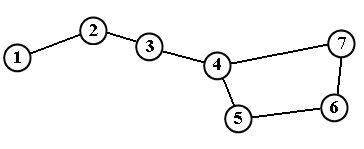
\includegraphics[width=8.641cm,height=3.542cm]{image/a2012Logique2eme-img047.jpg}
			\end{center}
			
		\subsubsection{Circuits et cycles}
		%=================================
			
			Dans un graphe orienté, un \textbf{circuit} est un chemin fermé, 
			c'est-à-dire une suite d'au minimum 2 arcs dont le n{\oe}ud de 
			départ est identique au n{\oe}ud d'arrivée. Pour un graphe non 
			orienté, on parle plutôt de \textbf{cycle}~:
			c'est également un chemin fermé constitué d'au moins 3 arêtes 
			adjacentes. Un circuit (ou un cycle) est \textbf{simple}
			ou \textbf{élémentaire} selon que le chemin correspondant 
			peut être qualifié de la même façon.

			Dans l'exemple ci-dessus, la suite d'arêtes 
			\{4, 5\}, \{5, 6\}, \{6, 7\}, \{7, 4\} 
			forme un cycle élémentaire de	longueur 4.

		\subsubsection{Connexité}
		%========================
		
		Un graphe \textbf{non orienté} est \textbf{connexe} 
		(ou \textbf{connecté}) s'il existe toujours un chemin 
		reliant deux n{\oe}uds quelconques de ce graphe. 
		Autrement dit, un graphe connexe est «~d'un seul tenant~».

		Une \textbf{composante connexe} d'un graphe est un sous-ensemble 
		de n{\oe}uds et d'arêtes de ce graphe formant lui-même
		un graphe connexe, et tel qu'il n'existe aucun chemin reliant 
		un de ses n{\oe}uds à un n{\oe}ud hors de ce sous-ensemble.

		Pour un graphe \textbf{orienté}, la définition de connexité est 
		analogue, toutefois en considérant les arcs sans leur orientation.

		Un graphe connexe ne possédant aucun cycle est un \textbf{arbre}, 
		et un graphe dont toutes les composantes connexes sont des arbres 
		est une \textbf{forêt}. Attention, ne pas confondre cette 
		définition d'arbre avec les arbres binaires et \textit{n}-aires 
		étudiés précédemment. Dans le contexte d'un graphe, il n'y a pas 
		de notion de racine, de niveau, de hauteur, de n{\oe}uds père et fils, etc. 
		Par contre, les n{\oe}uds d'un arbre qui sont de degré 1 portent aussi le
		nom de \textbf{feuilles}.

		\textbf{Exemple~:} Dans le graphe suivant, il y a trois composantes 
		connexes, respectivement formées par les sous-ensembles de n{\oe}uds 
		\{1, 2, 3, 4, 5, 6, 7, 8, 9\}, \{10, 11, 12\} et \{13, 14, 15\}. 
		La 3\textsuperscript{e} de ces composantes est un arbre.

		\begin{center}
		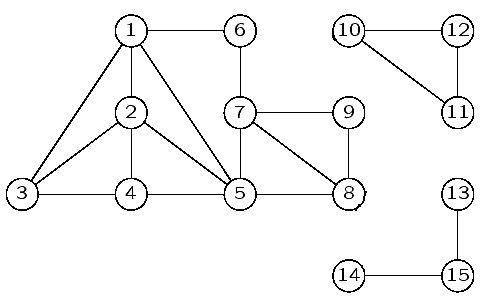
\includegraphics[width=6.235cm,height=3.955cm]{image/a2012Logique2eme-img048.jpg}
		\end{center}



%==================================
\section{Implémentation en mémoire}
%==================================

	\subsection{Représentation des n{\oe}uds}
	%========================================
				
		Dans les exemples précédents, les n{\oe}uds des graphes étaient 
		nommés par des lettres ou des numéros, mais ils peuvent
		contenir de l'information diverse. Par ex. dans le graphe 
		d'un réseau de métro, les n{\oe}uds seraient des chaines
		(noms des stations) ; en théorie des jeux, les n{\oe}uds 
		peuvent contenir la configuration complète de l'état d'un jeu,
		les arêtes représentant alors les possibilités de passage 
		d'une configuration à une autre. Le type des n{\oe}uds
		détermine le type du graphe~: on parlera d'un graphe d'entiers, 
		de chaines{\dots} et de façon générique, d'un graphe de type T.

		Le contenu des n{\oe}uds peut être stocké dans un tableau ou une 
		liste, selon le contexte. Un tableau convient bien pour
		implémenter un problème de graphe «~statique~» (où le nombre 
		de n{\oe}uds reste fixe) et la liste pour la modélisation
		d'un graphe qui subirait des transformations (ajout ou 
		suppression de n{\oe}uds). Dans tous les cas, on considère qu'il
		est toujours possible de numéroter les n{\oe}uds de 1 à \textit{n}.

	\subsection{Représentation des arcs/arêtes}
	%==========================================
				
		\subsubsection{Représentation matricielle}
		%=========================================

			La représentation matricielle est la façon la plus évidente 
			pour représenter les arêtes d'un graphe. Si seule
			l'existence des liens doit être représentée, on utilise une 
			matrice de booléens appelée \textbf{matrice d'adjacence}
			(ou \textbf{matrice de contigüité}). Chaque ligne et chaque 
			colonne de cette matrice correspond à un n{\oe}ud du
			graphe, conformément à la numérotation des n{\oe}uds choisie.

			Pour un graphe orienté, les lignes correspondent à l'origine des 
			arcs et les colonnes à leur extrémité. Ainsi, l'élément
			d'indices $(i, j)$ sera \textbf{vrai} si un arc 
			part de $i$ et arrive en $j$.

			\textbf{Exemple~:} Le graphe orienté ci-dessous à gauche 
			peut être représenté par la matrice d'adjacence à droite.

			\begin{center}
				\tablefirsthead{}
				\tablehead{}
				\tabletail{}
				\tablelasttail{}
				\begin{supertabular}{m{7.0350003cm}m{0.81600004cm}m{0.81600004cm}|m{0.81600004cm}|m{0.81600004cm}|m{0.81600004cm}|m{0.81600004cm}|m{0.81600004cm}|}
				\centering  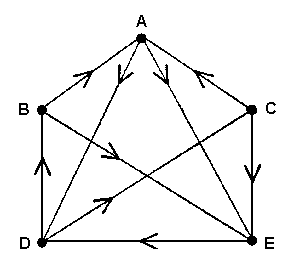
\includegraphics[width=4.318cm,height=3.859cm]{image/a2012Logique2eme-img049.png}  &
				~
				 &
				\multicolumn{1}{m{0.81600004cm}}{~
				} &
				\multicolumn{1}{m{0.81600004cm}}{\centering{ A}} &
				\multicolumn{1}{m{0.81600004cm}}{\centering{ B}} &
				\multicolumn{1}{m{0.81600004cm}}{\centering{ C}} &
				\multicolumn{1}{m{0.81600004cm}}{\centering{ D}} &
				\multicolumn{1}{m{0.81600004cm}}{\centering\arraybslash{ E}}\\\hhline{~~~-----}
				 &
				~
				 &
				\centering{ A} &
				\centering{ F} &
				\centering{ F} &
				\centering{ F} &
				\centering{ V} &
				\centering\arraybslash{ V}\\\hhline{~~~-----}
				 &
				~
				 &
				\centering{ B} &
				\centering{ V} &
				\centering{ F} &
				\centering{ F} &
				\centering{ F} &
				\centering\arraybslash{ V}\\\hhline{~~~-----}
				 &
				~
				 &
				\centering{ C} &
				\centering{ V} &
				\centering{ F} &
				\centering{ F} &
				\centering{ F} &
				\centering\arraybslash{ V}\\\hhline{~~~-----}
				 &
				~
				 &
				\centering{ D} &
				\centering{ F} &
				\centering{ V} &
				\centering{ V} &
				\centering{ F} &
				\centering\arraybslash{ F}\\\hhline{~~~-----}
				 &
				~
				 &
				\centering{ E} &
				\centering{ F} &
				\centering{ F} &
				\centering{ F} &
				\centering{ V} &
				\centering\arraybslash{ F}\\\hhline{~~~-----}
				 &
				~
				 &
				\multicolumn{1}{m{0.81600004cm}}{~
				} &
				\multicolumn{1}{m{0.81600004cm}}{~
				} &
				\multicolumn{1}{m{0.81600004cm}}{~
				} &
				\multicolumn{1}{m{0.81600004cm}}{~
				} &
				\multicolumn{1}{m{0.81600004cm}}{~
				} &
				\multicolumn{1}{m{0.81600004cm}}{~
				}\\
				\end{supertabular}
			\end{center}
			
			Dans le cas d'un graphe non orienté, l'élément d'indices $(i, j)$ 
			est mis à \textbf{vrai} si une arête rejoint les n{\oe}uds $i$ et $j$. 
			Comme cette relation est symétrique, la matrice d'adjacence qui en
			résulte est une \textbf{matrice symétrique}, c'est-à-dire que 
			$m_{ij} = m_{ji} \forall{i, j}$. Par économie, on peut aussi se limiter 
			dans ce cas à une \textbf{matrice triangulaire}, où seule une moitié 
			de la matrice est utilisée (par exemple les éléments $m{ij}$ 
			tels que $j \geq i$ s'il y a des boucles et $j > i$ sinon).

			\textbf{Exemple~:} Le graphe non orienté de la figure ci-dessous 
			peut être représenté par une matrice symétrique (à gauche) ou
			triangulaire supérieure (à droite).

			\begin{center}
			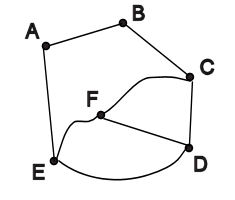
\includegraphics[width=3.784cm,height=3.233cm]{image/a2012Logique2eme-img050.jpg}
			\end{center}

			\begin{center}
				\tablefirsthead{}
				\tablehead{}
				\tabletail{}
				\tablelasttail{}
				\begin{supertabular}{m{0.93900007cm}|m{0.81600004cm}|m{0.81600004cm}|m{0.81600004cm}|m{0.81600004cm}|m{0.81600004cm}|m{0.81600004cm}|m{0.81600004cm}m{0.81600004cm}|m{0.81600004cm}|m{0.81600004cm}|m{0.81600004cm}|m{0.81600004cm}|m{0.81600004cm}|m{0.81600004cm}|}
				\multicolumn{1}{m{0.93900007cm}}{~
				} &
				\multicolumn{1}{m{0.81600004cm}}{\centering{ A}} &
				\multicolumn{1}{m{0.81600004cm}}{\centering{ B}} &
				\multicolumn{1}{m{0.81600004cm}}{\centering{ C}} &
				\multicolumn{1}{m{0.81600004cm}}{\centering{ D}} &
				\multicolumn{1}{m{0.81600004cm}}{\centering{ E}} &
				\multicolumn{1}{m{0.81600004cm}}{\centering{ F}} &
				~
				 &
				\multicolumn{1}{m{0.81600004cm}}{~
				} &
				\multicolumn{1}{m{0.81600004cm}}{\centering{ A}} &
				\multicolumn{1}{m{0.81600004cm}}{\centering{ B}} &
				\multicolumn{1}{m{0.81600004cm}}{\centering{ C}} &
				\multicolumn{1}{m{0.81600004cm}}{\centering{ D}} &
				\multicolumn{1}{m{0.81600004cm}}{\centering{ E}} &
				\multicolumn{1}{m{0.81600004cm}}{\centering\arraybslash{ F}}\\\hhline{~------~~------}
				\centering{ A} &
				\centering{ F} &
				\centering{ V} &
				\centering{ F} &
				\centering{ F} &
				\centering{ V} &
				\centering{ F} &
				~
				 &
				\centering{ A} &
				\centering{ F} &
				\centering{ V} &
				\centering{ F} &
				\centering{ F} &
				\centering{ V} &
				\centering\arraybslash{ F}\\\hhline{~------~~------}
				\centering{ B} &
				\centering{ V} &
				\centering{ F} &
				\centering{ V} &
				\centering{ F} &
				\centering{ F} &
				\centering{ F} &
				~
				 &
				\centering{ B} &
				\centering{ F} &
				\centering{ F} &
				\centering{ V} &
				\centering{ F} &
				\centering{ F} &
				\centering\arraybslash{ F}\\\hhline{~------~~------}
				\centering{ C} &
				\centering{ F} &
				\centering{ V} &
				\centering{ F} &
				\centering{ V} &
				\centering{ F} &
				\centering{ V} &
				~
				 &
				\centering{ C} &
				\centering{ F} &
				\centering{ F} &
				\centering{ F} &
				\centering{ V} &
				\centering{ F} &
				\centering\arraybslash{ V}\\\hhline{~------~~------}
				\centering{ D} &
				\centering{ F} &
				\centering{ F} &
				\centering{ V} &
				\centering{ F} &
				\centering{ V} &
				\centering{ V} &
				~
				 &
				\centering{ D} &
				\centering{ F} &
				\centering{ F} &
				\centering{ F} &
				\centering{ F} &
				\centering{ V} &
				\centering\arraybslash{ V}\\\hhline{~------~~------}
				\centering{ E} &
				\centering{ V} &
				\centering{ F} &
				\centering{ F} &
				\centering{ V} &
				\centering{ F} &
				\centering{ V} &
				~
				 &
				\centering{ E} &
				\centering{ F} &
				\centering{ F} &
				\centering{ F} &
				\centering{ F} &
				\centering{ F} &
				\centering\arraybslash{ V}\\\hhline{~------~~------}
				\centering{ F} &
				\centering{ F} &
				\centering{ F} &
				\centering{ V} &
				\centering{ V} &
				\centering{ V} &
				\centering{ F} &
				~
				 &
				\centering{ F} &
				\centering{ F} &
				\centering{ F} &
				\centering{ F} &
				\centering{ F} &
				\centering{ F} &
				\centering\arraybslash{ F}\\\hhline{~------~~------}
				\end{supertabular}
			\end{center}

			La représentation matricielle peut s'étendre aux cas des graphes 
			pondérés (en utilisant une matrice d'entiers contenant
			les poids des arêtes) ou d'un graphe étiqueté (matrice de chaines). 
			L'absence d'arc entre deux n{\oe}uds peut alors
			être signalée par des valeurs aberrantes (par exemple --1 
			ou «~infini~» pour des distances, «~rien~» pour le graphe
			étiqueté{\dots}).

			N.B.~: Quelle que soit la configuration choisie, la représentation 
			matricielle est cependant coûteuse en mémoire, car
			beaucoup d'éléments restent en général inoccupés. La matrice creuse 
			(voir ex. dans le chapitre sur les listes chainées)
			est plus appropriée à ce type de contenu.

		\subsubsection{Représentation par un tableau de listes}
		%======================================================
			
			L'idée est de faire correspondre à chaque n{\oe}ud la liste 
			des n{\oe}uds qui lui sont adjacents (pour un graphe
			orienté, ce sera la liste des n{\oe}uds pour lesquels un 
			arc part du n{\oe}ud considéré). Ces listes (qui peuvent
			éventuellement être chainées) sont contenues dans un tableau, 
			le \textbf{tableau des listes d'adjacence}, dont les
			indices correspondent à la numérotation des n{\oe}uds. 
			Les variantes de ce type de représentation sont nombreuses.

			L'avantage principal de cette représentation est le gain de 
			place en mémoire. Le désavantage est la perte de l'accès
			direct à l'information~: dans la matrice, on voit directement 
			si $i$ et $j$ sont adjacents, dans le cas du tableau, il faut 
			faire une recherche pour voir si $j$ se trouve dans la liste 
			d'indice $i$.

			\textbf{Exemple~:} voici une représentation du graphe orienté 
			de la page précédente sous forme de tableau de listes.
			\begin{center}
			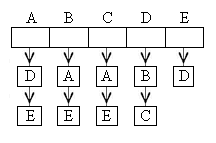
\includegraphics[width=5.715cm,height=3.784cm]{image/a2012Logique2eme-img051.png}
			\end{center}
			

%=========================
\section{Problèmes divers}
%=========================

	\subsection{Accessibilité d'un n{\oe}ud à partir d'un autre}
	%===========================================================

		Un n{\oe}ud $j$ est \textbf{accessible} à partir d'un n{\oe}ud $i$ 
		s'il existe un chemin partant de $i$ et arrivant à $j$. L'accessibilité 
		peut donc exister pour deux n{\oe}uds non adjacents. 
		Dans un graphe non orienté, l'accessibilité est assez évidente à établir~: 
		tous les n{\oe}uds d'une composante connexe du graphe sont forcément 
		accessibles. Le problème est moins immédiat et plus intéressant pour 
		les graphes orientés, et nous ne considérerons que ceux-ci 
		dans cette section.

		\subsubsection{Matrice d'accessibilité}
		%======================================

			Similairement à la matrice d'adjacence (qui indique si un n{\oe}ud 
			$i$ est en contact direct avec un n{\oe}ud $j$), la \textbf{matrice 
			d'accessibilité} est une matrice booléenne qui indique si à partir d'un 
			n{\oe}ud $i$, il existe un chemin qui mène au n{\oe}ud $j$. Comme 
			précédemment, l'indice ligne $i$ est associé à l'origine et l'indice 
			colonne $j$ à l'arrivée du chemin.

			\textbf{Exemple~:} Voici un graphe et sa matrice d'accessibilité. 
			On voit facilement que tous les n{\oe}uds sont accessibles à
			partir des n{\oe}uds 1 et 2. Par contre, les n{\oe}uds 3, 4 et 5 
			forment un cycle de longueur 3 duquel il n'est plus
			possible de retourner en 1 ou en 2.

			\begin{center}
				\tablefirsthead{}
				\tablehead{}
				\tabletail{}
				\tablelasttail{}
				\begin{supertabular}{m{7.0350003cm}m{0.81600004cm}m{0.81600004cm}m{0.81600004cm}|m{0.81600004cm}|m{0.81600004cm}|m{0.81600004cm}|m{0.81600004cm}|m{0.81600004cm}|}
				\centering  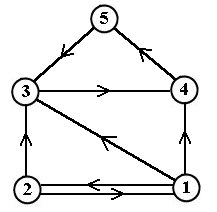
\includegraphics[width=4.355cm,height=4.247cm]{image/a2012Logique2eme-img052.jpg}  &
				~
				 &
				~
				 &
				\multicolumn{1}{m{0.81600004cm}}{~
				} &
				\multicolumn{1}{m{0.81600004cm}}{~
				} &
				\multicolumn{1}{m{0.81600004cm}}{~
				} &
				\multicolumn{1}{m{0.81600004cm}}{~
				} &
				\multicolumn{1}{m{0.81600004cm}}{~
				} &
				\multicolumn{1}{m{0.81600004cm}}{~
				}\\\hhline{~~~~-----}
				 &
				~
				 &
				~
				 &
				~
				 &
				\centering{ V} &
				\centering{ V} &
				\centering{ V} &
				\centering{ V} &
				\centering\arraybslash{ V}\\\hhline{~~~~-----}
				 &
				~
				 &
				~
				 &
				~
				 &
				\centering{ V} &
				\centering{ V} &
				\centering{ V} &
				\centering{ V} &
				\centering\arraybslash{ V}\\\hhline{~~~~-----}
				 &
				~
				 &
				~
				 &
				\centering{ \textit{A} =} &
				\centering{ F} &
				\centering{ F} &
				\centering{ V} &
				\centering{ V} &
				\centering\arraybslash{ V}\\\hhline{~~~~-----}
				 &
				~
				 &
				~
				 &
				~
				 &
				\centering{ F} &
				\centering{ F} &
				\centering{ V} &
				\centering{ V} &
				\centering\arraybslash{ V}\\\hhline{~~~~-----}
				 &
				~
				 &
				~
				 &
				~
				 &
				\centering{ F} &
				\centering{ F} &
				\centering{ V} &
				\centering{ V} &
				\centering\arraybslash{ V}\\\hhline{~~~~-----}
				 &
				~
				 &
				~
				 &
				\multicolumn{1}{m{0.81600004cm}}{~
				} &
				\multicolumn{1}{m{0.81600004cm}}{~
				} &
				\multicolumn{1}{m{0.81600004cm}}{~
				} &
				\multicolumn{1}{m{0.81600004cm}}{~
				} &
				\multicolumn{1}{m{0.81600004cm}}{~
				} &
				\multicolumn{1}{m{0.81600004cm}}{~
				}\\
				\end{supertabular}
			\end{center}
			
			Nous allons voir deux façons de générer la matrice d'accessibilité 
			en partant de la matrice d'adjacence d'un graphe.

		\subsubsection{Petit rappel de calcul matriciel}

			La somme de deux matrices de mêmes dimensions s'obtient en 
			additionnant les éléments de mêmes indices dans les deux
			matrices.
			
			Par exemple~:

			\begin{center}
				\tablefirsthead{}
				\tablehead{}
				\tabletail{}
				\tablelasttail{}
				\begin{supertabular}{|m{0.601cm}|m{0.601cm}|m{0.601cm}|m{0.601cm}m{0.601cm}m{0.601cm}|m{0.601cm}|m{0.601cm}|m{0.601cm}|m{0.601cm}m{0.601cm}m{0.601cm}|m{0.601cm}|m{0.601cm}|m{0.61800003cm}|}
				\hhline{---~~~---~~~---}
				\centering{ 1} &
				\centering{ 0} &
				\centering{ 4} &
				~
				 &
				~
				 &
				~
				 &
				\centering{ 3} &
				\centering{ 2} &
				\centering{ 1} &
				~
				 &
				~
				 &
				~
				 &
				\centering{ 4} &
				\centering{ 2} &
				\centering\arraybslash{ 5}\\\hhline{---~~~---~~~---}
				\centering{ {}--2} &
				\centering{ 2} &
				\centering{ 1} &
				~
				 &
				\centering{ +} &
				~
				 &
				\centering{ 2} &
				\centering{ 0} &
				\centering{ 3} &
				~
				 &
				\centering{ =} &
				~
				 &
				\centering{ 0} &
				\centering{ 2} &
				\centering\arraybslash{ 4}\\\hhline{---~~~---~~~---}
				\centering{ 3} &
				\centering{ 0} &
				\centering{ {}--1} &
				~
				 &
				~
				 &
				~
				 &
				\centering{ {}--2} &
				\centering{ 2} &
				\centering{ 0} &
				~
				 &
				~
				 &
				~
				 &
				\centering{ 1} &
				\centering{ 2} &
				\centering\arraybslash{ {}--1}\\\hhline{---~~~---~~~---}
				\end{supertabular}
			\end{center}

			La multiplication est un peu plus complexe~: 
			l'élément d'indices $(i, j)$ du produit de deux matrices
			est le \textit{produit scalaire} de la $i$\textsuperscript{e} 
			ligne de la première matrice par la $j$\textsuperscript{e} 
			colonne de la seconde. Le produit scalaire de deux vecteurs 
			(ou tableaux) de même taille est la somme des produits des 
			éléments de mêmes indices dans ces vecteurs. 
			
			En formule cela donne~:
			
			\begin{center}
			$(AB)_{ij} = \overset n{\underset{k=1}\sum} A_{ik} B_{kj}$
			\end{center}
			
			Attention, le produit matriciel n'est pas commutatif, 
			donc $AB \neq BA$ en général.

			\textbf{Exemple~:} pour obtenir l'élément d'indices (2, 1) 
			du produit, on calcule le produit scalaire de la
			2\textsuperscript{e} ligne de la 1\textsuperscript{ère} 
			matrice et de la 1\textsuperscript{ère} colonne de la
			2\textsuperscript{e}, soit $-2*3 + 2*2 + 1*(-2) = -4$.

			\begin{center}
				\tablefirsthead{}
				\tablehead{}
				\tabletail{}
				\tablelasttail{}
				\begin{supertabular}{|m{0.601cm}|m{0.601cm}|m{0.601cm}|m{0.601cm}m{0.601cm}m{0.601cm}|m{0.601cm}|m{0.601cm}|m{0.601cm}|m{0.601cm}m{0.601cm}m{0.601cm}|m{0.601cm}|m{0.601cm}|m{0.61800003cm}|}
				\hhline{---~~~---~~~---}
				\centering{ 1} &
				\centering{ 0} &
				\centering{ 4} &
				~
				 &
				~
				 &
				~
				 &
				\centering{ 3} &
				\centering{ 2} &
				\centering{ 1} &
				~
				 &
				~
				 &
				~
				 &
				\centering{ {}--5} &
				\centering{ 10} &
				\centering\arraybslash{ 1}\\\hhline{---~~~---~~~---}
				\centering{ {}--2} &
				\centering{ 2} &
				\centering{ 1} &
				~
				 &
				\centering{ *} &
				~
				 &
				\centering{ 2} &
				\centering{ 0} &
				\centering{ 3} &
				~
				 &
				\centering{ =} &
				~
				 &
				\centering{ {}--4} &
				\centering{ {}--2} &
				\centering\arraybslash{ 4}\\\hhline{---~~~---~~~---}
				\centering{ 3} &
				\centering{ 0} &
				\centering{ {}--1} &
				~
				 &
				~
				 &
				~
				 &
				\centering{ {}--2} &
				\centering{ 2} &
				\centering{ 0} &
				~
				 &
				~
				 &
				~
				 &
				\centering{ 11} &
				\centering{ 4} &
				\centering\arraybslash{ 3}\\\hhline{---~~~---~~~---}
				\end{supertabular}
			\end{center}

			Dans ce qui suit, nous serons amenés à calculer la somme 
			et le produit de matrices booléennes. Le calcul est analogue,
			en remplaçant toutefois les opérateurs + et * respectivement 
			par les opérateurs logiques OU et ET.

			\textbf{Exemple~:} somme et produit de deux matrices booléennes.

			\begin{center}
				\tablefirsthead{}
				\tablehead{}
				\tabletail{}
				\tablelasttail{}
				\begin{supertabular}{|m{0.601cm}|m{0.601cm}|m{0.601cm}|m{0.601cm}m{0.601cm}m{0.601cm}|m{0.601cm}|m{0.601cm}|m{0.601cm}|m{0.601cm}m{0.601cm}m{0.601cm}|m{0.601cm}|m{0.601cm}|m{0.61800003cm}|}
				\hhline{---~~~---~~~---}
				{ V} &
				{ F} &
				{ V} &
				~
				 &
				~
				 &
				~
				 &
				{ V} &
				{ V} &
				{ F} &
				~
				 &
				~
				 &
				~
				 &
				{ V} &
				{ V} &
				{ V}\\\hhline{---~~~---~~~---}
				{ V} &
				{ V} &
				{ F} &
				~
				 &
				{ +} &
				~
				 &
				{ V} &
				{ F} &
				{ V} &
				~
				 &
				{ =} &
				~
				 &
				{ V} &
				{ V} &
				{ V}\\\hhline{---~~~---~~~---}
				{ F} &
				{ V} &
				{ F} &
				~
				 &
				~
				 &
				~
				 &
				{ F} &
				{ F} &
				{ F} &
				~
				 &
				~
				 &
				~
				 &
				{ F} &
				{ V} &
				{ F}\\\hhline{---~~~---~~~---}
				\end{supertabular}
			\end{center}

			\begin{center}
				\tablefirsthead{}
				\tablehead{}
				\tabletail{}
				\tablelasttail{}
				\begin{supertabular}{|m{0.601cm}|m{0.601cm}|m{0.601cm}|m{0.601cm}m{0.601cm}m{0.601cm}|m{0.601cm}|m{0.601cm}|m{0.601cm}|m{0.601cm}m{0.601cm}m{0.601cm}|m{0.601cm}|m{0.601cm}|m{0.61800003cm}|}
				\hhline{---~~~---~~~---}
				{ V} &
				{ F} &
				{ V} &
				~
				 &
				~
				 &
				~
				 &
				{ V} &
				{ V} &
				{ F} &
				~
				 &
				~
				 &
				~
				 &
				{ V} &
				{ V} &
				{ F}\\\hhline{---~~~---~~~---}
				{ V} &
				{ V} &
				{ F} &
				~
				 &
				{ *} &
				~
				 &
				{ V} &
				{ F} &
				{ V} &
				~
				 &
				{ =} &
				~
				 &
				{ V} &
				{ V} &
				{ V}\\\hhline{---~~~---~~~---}
				{ F} &
				{ V} &
				{ F} &
				~
				 &
				~
				 &
				~
				 &
				{ F} &
				{ F} &
				{ F} &
				~
				 &
				~
				 &
				~
				 &
				{ V} &
				{ F} &
				{ V}\\\hhline{---~~~---~~~---}
				\end{supertabular}
			\end{center}

			Le premier élément du produit est obtenu en calculant \
			(V ET V) OU (F ET V) OU (V ET F) ${\equiv}$ V.

			À partir du produit matriciel, on définit encore l'élévation 
			à une puissance d'une matrice carrée (c'est-à-dire une
			matrice ayant autant de lignes que de colonnes)~: 
			$A^2 = A*A$, $A^3 = A*A^2$, et récursivement, $A^n = A*A^{n-1}$.
			
		\subsubsection{Puissances de la matrice d'adjacence}
		%===================================================

			Si $M$ est la matrice d'adjacence d'un graphe orienté, 
			alors la $k$\textsuperscript{e} puissance de
			$M$ possède la propriété suivante~: 
			$(M^k)_{ij}$ est vrai si et seulement s'il existe un chemin de 
			longueur $k$ partant de $i$ et arrivant à $j$.

			En effet, comme $(M^2)_{ij}=\overset n{\underset{k=1}\sum} M_{ik}\ast M_{kj}$, 
			cette somme donne vrai s'il existe au moins un $k$ pour lequel $M_{ik}$ et
			$M_{kj}$ sont vrais simultanément, autrement dit s'il existe un n{\oe}ud
			$k$ où arrive un arc partant de $i$, et d'où part un arc allant vers
			$j$, et donc s'il existe un chemin de longueur 2 entre $i$ et$j$. 
			Par récurrence, on prouve facilement que la propriété
			est valide pour les puissances suivantes.

			Supposons maintenant qu'au moins un élément $(i, j)$ 
			parmi les matrices $M$, $M^2$, $M^3$, ..., $M^n$ est vrai
			(où $n$ est le nombre de n{\oe}uds du graphe), 
			alors il existe au moins un chemin (de longueur maximale $n$) 
			entre les n{\oe}uds $i$ et $j$. On en déduit la formule suivante 
			pour la matrice	d'accessibilité~:

			\begin{center}
			$A=M+M^2+M^3+\cdots +M^n=\overset n{\underset{k=1}{\sum }}M^k$
			\end{center}
			
			\textbf{Exemple~:} calculons les puissances successives 
			de la matrice d'adjacence du graphe précédent~:

			\begin{center}
				\tablefirsthead{}
				\tablehead{}
				\tabletail{}
				\tablelasttail{}
				\begin{supertabular}{m{0.93900007cm}|m{0.81600004cm}|m{0.81600004cm}|m{0.81600004cm}|m{0.81600004cm}|m{0.81600004cm}|m{0.541cm}m{0.731cm}m{1.176cm}|m{0.81600004cm}|m{0.81600004cm}|m{0.81600004cm}|m{0.81600004cm}|m{0.83400005cm}|}
				\hhline{~-----~~~-----}
				~
				 &
				\centering{ F} &
				\centering{ V} &
				\centering{ V} &
				\centering{ V} &
				\centering{ F} &
				~
				 &
				~
				 &
				~
				 &
				\centering{ V} &
				\centering{ F} &
				\centering{ V} &
				\centering{ V} &
				\centering\arraybslash{ V}\\\hhline{~-----~~~-----}
				~
				 &
				\centering{ V} &
				\centering{ F} &
				\centering{ V} &
				\centering{ F} &
				\centering{ F} &
				~
				 &
				~
				 &
				~
				 &
				\centering{ F} &
				\centering{ V} &
				\centering{ V} &
				\centering{ V} &
				\centering\arraybslash{ F}\\\hhline{~-----~~~-----}
				\centering{ \textit{M}\textsuperscript{ }=} &
				\centering{ F} &
				\centering{ F} &
				\centering{ F} &
				\centering{ V} &
				\centering{ F} &
				~
				 &
				~
				 &
				\centering{ \textit{M}\textsuperscript{2 }=} &
				\centering{ F} &
				\centering{ F} &
				\centering{ F} &
				\centering{ F} &
				\centering\arraybslash{ V}\\\hhline{~-----~~~-----}
				~
				 &
				\centering{ F} &
				\centering{ F} &
				\centering{ F} &
				\centering{ F} &
				\centering{ V} &
				~
				 &
				~
				 &
				~
				 &
				\centering{ F} &
				\centering{ F} &
				\centering{ V} &
				\centering{ F} &
				\centering\arraybslash{ F}\\\hhline{~-----~~~-----}
				~
				 &
				\centering{ F} &
				\centering{ F} &
				\centering{ V} &
				\centering{ F} &
				\centering{ F} &
				~
				 &
				~
				 &
				~
				 &
				\centering{ F} &
				\centering{ F} &
				\centering{ F} &
				\centering{ V} &
				\centering\arraybslash{ F}\\\hhline{~-----~~~-----}
				\end{supertabular}
			\end{center}

			\begin{center}
				\tablefirsthead{}
				\tablehead{}
				\tabletail{}
				\tablelasttail{}
				\begin{supertabular}{m{0.93900007cm}|m{0.81600004cm}|m{0.81600004cm}|m{0.81600004cm}|m{0.81600004cm}|m{0.81600004cm}|m{0.541cm}m{0.731cm}m{1.176cm}|m{0.81600004cm}|m{0.81600004cm}|m{0.81600004cm}|m{0.81600004cm}|m{0.83400005cm}|}
				\hhline{~-----~~~-----}
				~
				 &
				\centering{ F} &
				\centering{ V} &
				\centering{ V} &
				\centering{ V} &
				\centering{ V} &
				~
				 &
				~
				 &
				~
				 &
				\centering{ V} &
				\centering{ F} &
				\centering{ V} &
				\centering{ V} &
				\centering\arraybslash{ V}\\\hhline{~-----~~~-----}
				~
				 &
				\centering{ V} &
				\centering{ F} &
				\centering{ V} &
				\centering{ V} &
				\centering{ V} &
				~
				 &
				~
				 &
				~
				 &
				\centering{ F} &
				\centering{ V} &
				\centering{ V} &
				\centering{ V} &
				\centering\arraybslash{ V}\\\hhline{~-----~~~-----}
				\centering{ \textit{M}\textsuperscript{3 }=} &
				\centering{ F} &
				\centering{ F} &
				\centering{ V} &
				\centering{ F} &
				\centering{ F} &
				~
				 &
				~
				 &
				\centering{ \textit{M}\textsuperscript{4 }=} &
				\centering{ F} &
				\centering{ F} &
				\centering{ F} &
				\centering{ V} &
				\centering\arraybslash{ F}\\\hhline{~-----~~~-----}
				~
				 &
				\centering{ F} &
				\centering{ F} &
				\centering{ F} &
				\centering{ V} &
				\centering{ F} &
				~
				 &
				~
				 &
				~
				 &
				\centering{ F} &
				\centering{ F} &
				\centering{ F} &
				\centering{ F} &
				\centering\arraybslash{ V}\\\hhline{~-----~~~-----}
				~
				 &
				\centering{ F} &
				\centering{ F} &
				\centering{ F} &
				\centering{ F} &
				\centering{ V} &
				~
				 &
				~
				 &
				~
				 &
				\centering{ F} &
				\centering{ F} &
				\centering{ V} &
				\centering{ F} &
				\centering\arraybslash{ F}\\\hhline{~-----~~~-----}
				\end{supertabular}
			\end{center}

			\begin{center}
				\tablefirsthead{}
				\tablehead{}
				\tabletail{}
				\tablelasttail{}
				\begin{supertabular}{m{0.93900007cm}|m{0.81600004cm}|m{0.81600004cm}|m{0.81600004cm}|m{0.81600004cm}|m{0.81600004cm}|m{0.541cm}m{0.731cm}m{1.176cm}m{0.81600004cm}m{0.81600004cm}m{0.81600004cm}m{0.81600004cm}m{0.81600004cm}}
				\hhline{~-----~~~~~~~~}
				~
				 &
				\centering{ F} &
				\centering{ V} &
				\centering{ V} &
				\centering{ V} &
				\centering{ V} &
				~
				 &
				~
				 &
				~
				 &
				~
				 &
				~
				 &
				~
				 &
				~
				 &
				~
				\\\hhline{~-----~~~~~~~~}
				~
				 &
				\centering{ V} &
				\centering{ F} &
				\centering{ V} &
				\centering{ V} &
				\centering{ V} &
				~
				 &
				~
				 &
				~
				 &
				~
				 &
				~
				 &
				~
				 &
				~
				 &
				~
				\\\hhline{~-----~~~~~~~~}
				\centering{ \textit{M}\textsuperscript{5 }=} &
				\centering{ F} &
				\centering{ F} &
				\centering{ F} &
				\centering{ F} &
				\centering{ V} &
				~
				 &
				~
				 &
				~
				 &
				~
				 &
				~
				 &
				~
				 &
				~
				 &
				~
				\\\hhline{~-----~~~~~~~~}
				~
				 &
				\centering{ F} &
				\centering{ F} &
				\centering{ V} &
				\centering{ F} &
				\centering{ F} &
				~
				 &
				~
				 &
				~
				 &
				~
				 &
				~
				 &
				~
				 &
				~
				 &
				~
				\\\hhline{~-----~~~~~~~~}
				~
				 &
				\centering{ F} &
				\centering{ F} &
				\centering{ F} &
				\centering{ V} &
				\centering{ F} &
				~
				 &
				~
				 &
				~
				 &
				~
				 &
				~
				 &
				~
				 &
				~
				 &
				~
				\\\hhline{~-----~~~~~~~~}
				\end{supertabular}
			\end{center}
			
			On vérifie facilement qu'en additionnant (logiquement) les 5 matrices, 
			on obtient bien la matrice d'accessibilité.

			\textbf{Remarques.}

			\begin{enumerate}
				\item {
					Si on travaille avec des matrices à valeurs entières plutôt 
					que booléennes (c'est-à-dire avec 1 pour \textbf{vrai} et
					0 pour \textbf{faux}), $(M^k)_{ij}$ représente alors le nombre
					de chemins de longueur $k$ allant de $i$ à $j$. La somme 
					des puissances de la matrice d'adjacence donne alors le nombre 
					de chemins allant de $i$ à $j$ de longueur~inférieure ou égale à
					$n$ (nombre de n{\oe}uds).}
				\item {
					L'algorithme qui découle de cette formule ne présente aucune 
					difficulté d'élaboration. Il est cependant moins performant
					que celui de Roy-Warshall que nous présentons ci-dessous.}
				\item {
					Le graphe obtenu à partir de la matrice d'accessibilité 
					s'appelle la \textbf{fermeture transitive} du graphe de départ
					ou encore \textbf{graphe d'accessibilité}.}
			\end{enumerate}
			
		\subsubsection{Algorithme de Roy-Warshall}

			Soit $P_k$ la matrice booléenne définie de la façon suivante~:
			$P_k[i, j] = \textbf{vrai}$ s'il existe un chemin du n{\oe}ud
			$i$ au n{\oe}ud $j$ dont les indices des autres n{\oe}uds 
			valent au maximum $k$ (autrement dit, qui n'utilise aucun autre 
			n{\oe}ud intermédiaire que ceux d'indices 1 à $k$). Cette matrice 
			est définie pour les valeurs de $k$ entre 0 et $n$ inclus 
			($n$ étant le nombre de n{\oe}uds).

			Il résulte de cette définition que $P_0$ est la matrice d'adjacence 
			et que $P_n$ est la matrice d'accessibilité. L'algorithme de Roy-Warshall 
			permet de calculer facilement $P_k$ à partir de $P_{k-1}$,
			et donc d'accéder en $n$ étapes à la matrice d'accessibilité. 
			La règle de récurrence est la suivante~:

			\begin{center}
				$P_k[i, j]$ est vrai $\Leftrightarrow$ $P_{k-1}[i, j]$ est vrai OU 
				($P_{k-1}[i, k]$ ET $P_{k-1}[k, j]$ sont vrais)
			\end{center}

			En effet, si $P_{k-1}[i, j]$ est vrai, $P_{k}[i, j]$ l'est forcément. 
			Si $P_{k-1}[i, k]$ et $P_{k-1}[k,	j]$ sont tous deux vrais, 
			cela veut dire qu'il existe un chemin allant de $i$ à $k$, et un autre
			allant de $k$ à $j$, chacun n'utilisant que les n{\oe}uds d'indices 
			valant au maximum $k-1$. En mettant ces deux chemins bout à bout, 
			on obtient bien un chemin de $i$ à $j$ dont les indices des
			n{\oe}uds sont au maximum $k$.

			Un des avantages de l'algorithme est de pouvoir calculer les matrices 
			$P_k$ dans un seul tableau. Une fois qu'un élément [i, j] est vrai, 
			il reste vrai à toutes les étapes restantes. Le code de l'algorithme
			est le suivant~:
			
			\cadre{
				\begin{pseudo}
					\Module{RoyWarshall}{M\In, P\Out~: tableaux[1 à n, 1 à n] de booléens}{}
						\Decl i, j, k~: entiers
						\Let P \Gets M 
						\RComment initialisation de P avec une copie de la matrice d'adjacence
						\For{k \K{de} 1 \K{à} n}
							\LComment calcul des éléments de $P_{k}$
							\For{i \K{de} 1 \K{à} n}
								\For{j \K{de} 1 \K{à} n}
									\Let P[i, j] \Gets P[i, j] \K{ou} (P[i, k] \K{et} P[k, j])
								\EndFor
							\EndFor
						\EndFor
					\LComment  P contient à présent la matrice d'accessibilité
					\EndModule
				\end{pseudo}
			}

			\textbf{Exemple~:} Toujours pour le même graphe, voici les états 
			successifs de la matrice obtenue par l'algorithme de Roy-Warshall. 
			Les nouveaux éléments devenus à vrai sont indiqués en grisé.

			\begin{center}
				\tablefirsthead{}
				\tablehead{}
				\tabletail{}
				\tablelasttail{}
				\begin{supertabular}{m{0.93900007cm}|m{0.81600004cm}|m{0.81600004cm}|m{0.81600004cm}|m{0.81600004cm}|m{0.81600004cm}|m{0.541cm}m{0.731cm}m{1.176cm}|m{0.81600004cm}|m{0.81600004cm}|m{0.81600004cm}|m{0.81600004cm}|m{0.83400005cm}|}
				\hhline{~-----~~~-----}
				~
				 &
				\centering{ F} &
				\centering{ V} &
				\centering{ V} &
				\centering{ V} &
				\centering{ F} &
				~
				 &
				~
				 &
				~
				 &
				\centering{ F} &
				\centering{ V} &
				\centering{ V} &
				\centering{ V} &
				\centering\arraybslash{ F}\\\hhline{~-----~~~-----}
				~
				 &
				\centering{ V} &
				\centering{ F} &
				\centering{ V} &
				\centering{ F} &
				\centering{ F} &
				~
				 &
				~
				 &
				~
				 &
				\centering{ V} &
				\centering{ \cellcolor{gray!25}V} &
				\centering{ V} &
				\centering{ \cellcolor{gray!25}V} &
				\centering\arraybslash{ F}\\\hhline{~-----~~~-----}
				\centering{ $P_0$ =} &
				\centering{ F} &
				\centering{ F} &
				\centering{ F} &
				\centering{ V} &
				\centering{ F} &
				~
				 &
				~
				 &
				\centering{ $P_1$ =} &
				\centering{ F} &
				\centering{ F} &
				\centering{ F} &
				\centering{ V} &
				\centering\arraybslash{ F}\\\hhline{~-----~~~-----}
				~
				 &
				\centering{ F} &
				\centering{ F} &
				\centering{ F} &
				\centering{ F} &
				\centering{ V} &
				~
				 &
				~
				 &
				~
				 &
				\centering{ F} &
				\centering{ F} &
				\centering{ F} &
				\centering{ F} &
				\centering\arraybslash{ V}\\\hhline{~-----~~~-----}
				~
				 &
				\centering{ F} &
				\centering{ F} &
				\centering{ V} &
				\centering{ F} &
				\centering{ F} &
				~
				 &
				~
				 &
				~
				 &
				\centering{ F} &
				\centering{ F} &
				\centering{ V} &
				\centering{ F} &
				\centering\arraybslash{ F}\\\hhline{~-----~~~-----}
				\end{supertabular}
			\end{center}

			\bigskip

			\begin{center}
				\tablefirsthead{}
				\tablehead{}
				\tabletail{}
				\tablelasttail{}
				\begin{supertabular}{m{0.93900007cm}|m{0.81600004cm}|m{0.81600004cm}|m{0.81600004cm}|m{0.81600004cm}|m{0.81600004cm}|m{0.541cm}m{0.731cm}m{1.176cm}|m{0.81600004cm}|m{0.81600004cm}|m{0.81600004cm}|m{0.81600004cm}|m{0.83400005cm}|}
				\hhline{~-----~~~-----}
				~
				 &
				\centering{ \cellcolor{gray!25}V} &
				\centering{ V} &
				\centering{ V} &
				\centering{ V} &
				\centering{ F} &
				~
				 &
				~
				 &
				~
				 &
				\centering{ V} &
				\centering{ V} &
				\centering{ V} &
				\centering{ V} &
				\centering\arraybslash{ F}\\\hhline{~-----~~~-----}
				~
				 &
				\centering{ V} &
				\centering{ V} &
				\centering{ V} &
				\centering{ V} &
				\centering{ F} &
				~
				 &
				~
				 &
				~
				 &
				\centering{ V} &
				\centering{ V} &
				\centering{ V} &
				\centering{ V} &
				\centering\arraybslash{ F}\\\hhline{~-----~~~-----}
				\centering{ $P_2$ =} &
				\centering{ F} &
				\centering{ F} &
				\centering{ F} &
				\centering{ V} &
				\centering{ F} &
				~
				 &
				~
				 &
				\centering{ $P_3$ =} &
				\centering{ F} &
				\centering{ F} &
				\centering{ F} &
				\centering{ V} &
				\centering\arraybslash{ F}\\\hhline{~-----~~~-----}
				~
				 &
				\centering{ F} &
				\centering{ F} &
				\centering{ F} &
				\centering{ F} &
				\centering{ V} &
				~
				 &
				~
				 &
				~
				 &
				\centering{ F} &
				\centering{ F} &
				\centering{ F} &
				\centering{ F} &
				\centering\arraybslash{ V}\\\hhline{~-----~~~-----}
				~
				 &
				\centering{ F} &
				\centering{ F} &
				\centering{ V} &
				\centering{ F} &
				\centering{ F} &
				~
				 &
				~
				 &
				~
				 &
				\centering{ F} &
				\centering{ F} &
				\centering{ V} &
				\centering{ \cellcolor{gray!25}V} &
				\centering\arraybslash{ F}\\\hhline{~-----~~~-----}
				\end{supertabular}
			\end{center}

			\bigskip

			\begin{center}
				\tablefirsthead{}
				\tablehead{}
				\tabletail{}
				\tablelasttail{}
				\begin{supertabular}{m{0.93900007cm}|m{0.81600004cm}|m{0.81600004cm}|m{0.81600004cm}|m{0.81600004cm}|m{0.81600004cm}|m{0.541cm}m{0.731cm}m{1.176cm}|m{0.81600004cm}|m{0.81600004cm}|m{0.81600004cm}|m{0.81600004cm}|m{0.83400005cm}|}
				\hhline{~-----~~~-----}
				~
				 &
				\centering{ V} &
				\centering{ V} &
				\centering{ V} &
				\centering{ V} &
				\centering{ \cellcolor{gray!25}V} &
				~
				 &
				~
				 &
				~
				 &
				\centering{ V} &
				\centering{ V} &
				\centering{ V} &
				\centering{ V} &
				\centering\arraybslash{ V}\\\hhline{~-----~~~-----}
				~
				 &
				\centering{ V} &
				\centering{ V} &
				\centering{ V} &
				\centering{ V} &
				\centering{ \cellcolor{gray!25}V} &
				~
				 &
				~
				 &
				~
				 &
				\centering{ V} &
				\centering{ V} &
				\centering{ V} &
				\centering{ V} &
				\centering\arraybslash{ V}\\\hhline{~-----~~~-----}
				\centering{ $P_4$ =} &
				\centering{ F} &
				\centering{ F} &
				\centering{ F} &
				\centering{ V} &
				\centering{ \cellcolor{gray!25}V} &
				~
				 &
				~
				 &
				\centering{ $P_5$ =} &
				\centering{ F} &
				\centering{ F} &
				\centering{ \cellcolor{gray!25}V} &
				\centering{ V} &
				\centering\arraybslash{ V}\\\hhline{~-----~~~-----}
				~
				 &
				\centering{ F} &
				\centering{ F} &
				\centering{ F} &
				\centering{ F} &
				\centering{ V} &
				~
				 &
				~
				 &
				~
				 &
				\centering{ F} &
				\centering{ F} &
				\centering{ \cellcolor{gray!25}V} &
				\centering{ \cellcolor{gray!25}V} &
				\centering\arraybslash{ V}\\\hhline{~-----~~~-----}
				~
				 &
				\centering{ F} &
				\centering{ F} &
				\centering{ V} &
				\centering{ V} &
				\centering{ \cellcolor{gray!25}V} &
				~
				 &
				~
				 &
				~
				 &
				\centering{ F} &
				\centering{ F} &
				\centering{ V} &
				\centering{ V} &
				\centering\arraybslash{ V}\\\hhline{~-----~~~-----}
				\end{supertabular}
			\end{center}
	
	\subsection{Problèmes d'optimisation}
	%====================================
				
		Ce type de problèmes s'applique aux graphes pondérés, 
		orientés ou non. Il en existe beaucoup de variantes~:
		détermination du chemin de poids ou de coût minimum, 
		de la distance minimale ou du chemin le plus court entre deux
		n{\oe}uds d'un graphe, du chemin de poids minimum passant 
		par tous les n{\oe}uds d'un graphe (problème du voyageur de
		commerce), la recherche de l'arbre de poids minimum 
		inclus dans un graphe (algorithme de Kruskal), etc.

		Pour représenter un graphe pondéré, on utilise une matrice 
		des poids (entiers ou réels) $W$, ou $W_{ij}$ est
		une valeur positive représentant le poids de l'arc existant 
		entre les n{\oe}uds $i$ et $j$. L'absence d'arc doit être signalée 
		par une valeur aberrante, qui selon le contexte peut être négative, 
		nulle ou infinie. Dans le cas de la recherche du minimum, les arcs 
		inexistants doivent être initialisés à une valeur «~infinie~» (plus
		techniquement une constante du type \textit{highest value}).

		Une légère modification de l'algorithme de Roy-Warshall permet de 
		construire la matrice $P$ des poids minimum entre les différents
		n{\oe}uds d'un graphe. À l'étape $k$, on compare la valeur $P_{ij}$
		connue jusque là avec le poids d'un chemin passant par le n{\oe}ud $k$. 
		Si ce détour s'avère plus coûteux, on garde $P_{ij}$ ; 
		si par contre le détour par le n{\oe}ud \textit{k} allège le poids, 
		$P_{ij}$ est remplacé alors par le poids de ce nouveau chemin, 
		soit $P_{ik} + P_{kj}$. 
		
		\cadre{
			\begin{pseudo}
				\Module{poidsMinimum}{W\In, P\Out~: tableaux[1 à n, 1 à n] d'entiers}{}
				\RComment réels
					\Decl i, j, k~: entiers
					\Let P \Gets W 
					\RComment initialisation de P avec une copie de la matrice des poids
					\For{k \K{de} 1 \K{à} n}
						\For{i \K{de} 1 \K{à} n}
							\For{j \K{de} 1 \K{à} n}
								\Let P[i, j] \Gets min(P[i, j], P[i, k] + P[k, j])
							\EndFor
						\EndFor
					\EndFor
					\LComment P contient à présent la matrice des poids minimum
				\EndModule
			\end{pseudo}
		}

		\textbf{Exemple~:} Voici pour le graphe suivant les contenus des matrices 
		obtenues à chaque étape de l'algorithme de recherche des poids minimum. 

		\begin{center}
		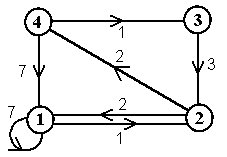
\includegraphics[width=5.5cm,height=3.782cm]{image/a2012Logique2eme-img053.jpg}
		\end{center}

		\begin{center}
			\tablefirsthead{}
			\tablehead{}
			\tabletail{}
			\tablelasttail{}
			\begin{supertabular}{|m{0.40000004cm}|m{0.40000004cm}|m{0.40000004cm}|m{0.40000004cm}|m{0.611cm}|m{0.435cm}|m{0.454cm}|m{0.40000004cm}|m{0.40000004cm}|m{0.486cm}|m{0.435cm}|m{0.58cm}|m{0.40000004cm}|m{0.537cm}|m{0.56200004cm}|m{0.52000004cm}|m{0.435cm}|m{0.435cm}|m{0.435cm}|m{0.47400004cm}|m{0.40000004cm}|m{0.40000004cm}|m{0.40000004cm}|m{0.426cm}|}
			\multicolumn{4}{m{2.2cm}}{\centering{ état initial}} &
			\multicolumn{1}{m{0.611cm}}{~
			} &
			\multicolumn{4}{m{2.289cm}}{\centering{ k=1}} &
			\multicolumn{1}{m{0.486cm}}{~
			} &
			\multicolumn{4}{m{2.5519998cm}}{\centering{ k=2}} &
			\multicolumn{1}{m{0.56200004cm}}{~
			} &
			\multicolumn{4}{m{2.425cm}}{\centering{ k=3}} &
			\multicolumn{1}{m{0.47400004cm}}{~
			} &
			\multicolumn{4}{m{2.226cm}}{\centering{ k=4}}\\\hhline{----~----~----~----~----}
			\centering{ 7} &
			\centering{ 1} &
			\centering{ ${\infty}$} &
			\centering{ ${\infty}$} &
			~
			 &
			\centering{ 7} &
			\centering{ 1} &
			\centering{ ${\infty}$} &
			\centering{ ${\infty}$} &
			~
			 &
			\centering{ 3} &
			\centering{ 1} &
			\centering{ ${\infty}$} &
			\centering{ 3} &
			~
			 &
			\centering{ 3} &
			\centering{ 1} &
			\centering{ ${\infty}$} &
			\centering{ 3} &
			~
			 &
			\centering{ 3} &
			\centering{ 1} &
			{ 4} &
			\centering\arraybslash{ 3}\\\hhline{----~----~----~----~----}
			\centering{ 2} &
			\centering{ ${\infty}$} &
			\centering{ ${\infty}$} &
			\centering{ 2} &
			~
			 &
			\centering{ 2} &
			\centering{ 3} &
			\centering{ ${\infty}$} &
			\centering{ 2} &
			~
			 &
			\centering{ 2} &
			\centering{ 3} &
			\centering{ ${\infty}$} &
			\centering{ 2} &
			~
			 &
			\centering{ 2} &
			\centering{ 3} &
			\centering{ ${\infty}$} &
			\centering{ 2} &
			~
			 &
			\centering{ 2} &
			\centering{ 3} &
			{ 3} &
			\centering\arraybslash{ 2}\\\hhline{----~----~----~----~----}
			\centering{ ${\infty}$} &
			\centering{ 3} &
			\centering{ ${\infty}$} &
			\centering{ ${\infty}$} &
			~
			 &
			\centering{ ${\infty}$} &
			\centering{ 3} &
			\centering{ ${\infty}$} &
			\centering{ ${\infty}$} &
			~
			 &
			\centering{ 5} &
			\centering{ 3} &
			\centering{ ${\infty}$} &
			\centering{ 5} &
			~
			 &
			\centering{ 5} &
			\centering{ 3} &
			\centering{ ${\infty}$} &
			\centering{ 5} &
			~
			 &
			\centering{ 5} &
			\centering{ 3} &
			{ 6} &
			\centering\arraybslash{ 5}\\\hhline{----~----~----~----~----}
			\centering{ 7} &
			\centering{ ${\infty}$} &
			\centering{ 1} &
			\centering{ ${\infty}$} &
			~
			 &
			\centering{ 7} &
			\centering{ 8} &
			\centering{ 1} &
			\centering{ ${\infty}$} &
			~
			 &
			\centering{ 6} &
			\centering{ 8} &
			\centering{ 1} &
			\centering{ 10} &
			~
			 &
			\centering{ 6} &
			\centering{ 4} &
			\centering{ 1} &
			\centering{ 6} &
			~
			 &
			\centering{ 6} &
			\centering{ 4} &
			{ 1} &
			\centering\arraybslash{ 6}\\\hhline{----~----~----~----~----}
			\end{supertabular}
		\end{center}

		\textbf{Remarque.} L'algorithme ci-dessus détermine les poids 
		minimum entre toutes les paires de n{\oe}uds du graphe. Il existe
		de nombreuses variantes, dont l'\textbf{algorithme de Dijkstra} 
		qui recherche les poids uniquement entre un n{\oe}ud
		donné et les autres n{\oe}uds du graphe. Cet algorithme utilise 
		seulement un tableau de $n$ valeurs (au lieu d'une matrice $n$ x $n$).

	\subsection{Parcours d'un graphe}
	%================================
		
		Comment parcourir les n{\oe}uds d'un graphe ? Plusieurs solutions sont 
		possibles. On pourrait bien sûr les parcourir dans l'ordre de leur 
		énumération, mais ce parcours ne tiendrait pas compte des liens 
		entre les n{\oe}uds. Deux parcours particuliers apparaissent dans 
		la théorie des graphes, selon le type de problème à résoudre~: 
		le parcours \textit{par contagion} et le parcours \textit{par sondage}.

		Au cours de l'exécution des algorithmes correspondant à ces parcours, 
		chaque n{\oe}ud sera dans un des 3 états suivants~: 
		\textbf{Prêt} (état initial), \textbf{Attente }(en attente d'être traité) 
		ou \textbf{Traité}.

		Ces états peuvent être stockés dans un tableau de chaines, 
		ou éventuellement de booléens (en assimilant les états
		\textbf{Attente} et \textbf{Traité} en un seul état 
		«~\textbf{Visité}~»). Dans les deux algorithmes ci-dessous, 
		la détermination des n{\oe}uds voisins est très aisée, que 
		ce soit par la matrice d'adjacence ou par le tableau de listes.
		Les algorithmes sont rédigés en «~macro-logique~», afin de 
		pouvoir les adapter facilement selon le choix de la
		représentation choisie.

		\subsubsection{Parcours par contagion}
		%=====================================
			
			À partir d'un n{\oe}ud de départ, on visite d'abord ses voisins, 
			puis les voisins des voisins et ainsi de suite{\dots}
			On visite donc le graphe par «~couches~», d'abord les voisins 
			dans l'entourage immédiat, puis on s'éloigne petit à
			petit de plus en plus loin{\dots}

			\cadre{
				\begin{pseudo}
					\Module{ParcoursContagion}{départ, ...}{} 
					\RComment la représentation du graphe n'est pas précisée ici
						\LComment initialiser tous les états des n{\oe}uds à prêt
						\Let état de départ \Gets Attente
						\Stmt file.enfiler(départ)
						\While{NON file.estVide( )}
							\Let n{\oe}ud \Gets file.défiler( )
							\LComment traitement du n{\oe}ud
							\Let état de n{\oe}ud \Gets Traité
							\For{tous les voisins de n{\oe}uds}
								\If{état de voisin = Prêt}
									\Let état de voisin \Gets Attente
									\Stmt file.enfiler(voisin)
								\EndIf
							\EndFor
						\EndWhile
					\EndModule
				\end{pseudo}
			}
			
		\subsubsection{Parcours par sondage}
		%===================================
			
			L'algorithme est semblable au précédent, à part que l'on 
			utilise ici une pile au lieu d'une file. Il en résulte le
			parcours suivant~: à partir du n{\oe}ud de départ, on 
			visite un voisin, puis immédiatement un voisin de ce voisin et
			ainsi de suite, on s'éloigne le plus loin possible jusqu'à un 
			premier cul-de-sac. On revient alors en arrière et on
			recommence dans la première voie non encore visitée.

			\cadre{
				\begin{pseudo}
					\Module{ParcoursSondage}{départ, ...}{}
					\RComment la représentation du graphe n'est pas précisée ici
						\LComment initialiser tous les états des n{\oe}uds à prêt
						\Let état de départ \Gets Attente
						\Stmt pile.empiler(départ)
						\While{NON pile.estVide( )}
							\Let n{\oe}ud \Gets pile.dépiler( )
							\LComment traitement du n{\oe}ud
							\Let état de n{\oe}ud \Gets Traité
								\For{tous les voisins de n{\oe}uds}
									\If{état de voisin = Prêt}
										\Let état de voisin \Gets Attente
										\Stmt pile.empiler(voisin)
									\EndIf
								\EndFor
							\EndWhile
						\EndModule
					\end{pseudo}
				}

			\textbf{Remarque.} Noter que dans ces algorithmes, il n'y a pas 
			de contrainte sur l'ordre de visite des voisins, celui-ci
			dépendra en partie de l'énumération des n{\oe}uds 
			choisie ou du parcours des listes d'adjacence.

			\textbf{Exemple~:} Dans le graphe suivant, en supposant que les 
			voisins soient parcourus dans l'ordre des listes du tableau, le
			parcours par contagion à partir de A donnera A, D, E, B, C et 
			le parcours par sondage A, E, D, C, B.

			\begin{center}
			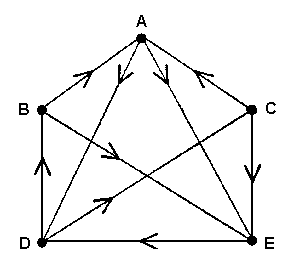
\includegraphics[width=4.99cm,height=4.473cm]{image/a2012Logique2eme-img054.png}  \ \ \ \ \ \ \ \ \ \ \ \ \ 
			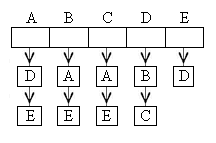
\includegraphics[width=5.715cm,height=3.784cm]{image/a2012Logique2eme-img055.png} 
			\end{center}


%==================
\section{Exercices}
%==================

	\begin{Exercice}{}
		Soit un graphe orienté dont la matrice d'adjacence est la suivante~:
				
		\begin{center}
			\tablefirsthead{}
			\tablehead{}
			\tabletail{}
			\tablelasttail{}
			\begin{supertabular}{m{0.93900007cm}|m{0.81600004cm}|m{0.81600004cm}|m{0.81600004cm}|m{0.81600004cm}|m{0.81600004cm}|}
			\multicolumn{1}{m{0.93900007cm}}{~
			} &
			\multicolumn{1}{m{0.81600004cm}}{\centering{ A}} &
			\multicolumn{1}{m{0.81600004cm}}{\centering{ B}} &
			\multicolumn{1}{m{0.81600004cm}}{\centering{ C}} &
			\multicolumn{1}{m{0.81600004cm}}{\centering{ D}} &
			\multicolumn{1}{m{0.81600004cm}}{\centering\arraybslash{ E}}\\\hhline{~-----}
			\centering{ A} &
			\centering{ F} &
			\centering{ V} &
			\centering{ F} &
			\centering{ V} &
			\centering\arraybslash{ F}\\\hhline{~-----}
			\centering{ B} &
			\centering{ F} &
			\centering{ F} &
			\centering{ V} &
			\centering{ F} &
			\centering\arraybslash{ F}\\\hhline{~-----}
			\centering{ C} &
			\centering{ V} &
			\centering{ F} &
			\centering{ F} &
			\centering{ F} &
			\centering\arraybslash{ F}\\\hhline{~-----}
			\centering{ D} &
			\centering{ F} &
			\centering{ F} &
			\centering{ F} &
			\centering{ F} &
			\centering\arraybslash{ V}\\\hhline{~-----}
			\centering{ E} &
			\centering{ V} &
			\centering{ F} &
			\centering{ F} &
			\centering{ F} &
			\centering\arraybslash{ F}\\\hhline{~-----}
			\end{supertabular}
		\end{center}
		
		\begin{enumerate}
			\item {
				Dessiner le graphe correspondant}
			\item {
				Établir la matrice d'accessibilité par l'algorithme de Roy-Warshall}
			\item {
				Que représente la matrice obtenue à la 3\textsuperscript{e} étape de cet algorithme ?}
		\end{enumerate}
		
	\end{Exercice}
	
	\begin{Exercice}{}
		Un graphe orienté est représenté par un tableau de 
		listes d'adjacence. Le contenu de ce tableau est
		(2), ( ), (1,3), (2, 4), (3, 5, 7), (4, 6), (5, 7), (4, 6). 
		Dessiner un graphe correspondant.

	\end{Exercice}
	
	\begin{Exercice}{}
		Soit le graphe orienté suivant~:
		
		\begin{center}
		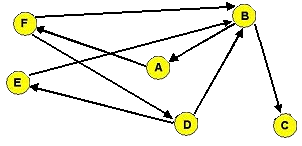
\includegraphics[width=6.854cm,height=3.318cm]{image/a2012Logique2eme-img056.png}
		\end{center}

		\begin{itemize}
			\item {
				Donner sa matrice d'adjacence, en faisant correspondre les lettres 
				prises dans l'ordre alphabétique aux indices pris
				dans l'ordre croissant.}
			\item {
				Ce graphe est-il complet? Expliquer.}
			\item {
				Ce graphe contient-il des n{\oe}uds particuliers? Si oui, lesquels.}
			\item {
				Existe-t-il un chemin reliant B à E ? Si oui lequel. 
				Dans quelle étape de l'algorithme de Roy-Warshall ce chemin
				apparait-il ? }
			\item {
				Que donne l'énumération des valeurs des n{\oe}uds donnée 
				par contagion à partir du n{\oe}ud F ? }
			\item {
				Même question par sondage.}
		\end{itemize}

	\end{Exercice}
	
	\begin{Exercice}{}
		Soit un graphe orienté à $n$ n{\oe}uds (avec $n>1$). 
		Comment relier ces n{\oe}uds avec le nombre minimum d'arcs pour 
		obtenir un graphe dont la matrice d'accessibilité ne contienne 
		que des 1 ? Quel est le nombre minimum d'arcs requis ?

	\end{Exercice}
	
	\begin{Exercice}{}
		Est-il possible que la matrice d'accessibilité 
		d'un graphe soit identique à sa matrice d'adjacence ?
	\end{Exercice}
	
	\begin{Exercice}{}
		Soit un graphe non orienté donné par sa matrice d'adjacence 
		(a) symétrique (b) triangulaire supérieure. 
		Écrire un algorithme qui détermine le n{\oe}ud de plus grand 
		degré de ce graphe. En cas d'ex-æquo, on retournera le n{\oe}ud de
		plus petit indice.

	\end{Exercice}
	
	\begin{Exercice}{}
		Soit un graphe non orienté donné par sa matrice d'adjacence. 
		Écrire un algorithme qui détermine le nombre de
		sous-composantes connexes de ce graphe. \
		Même question pour un graphe orienté.

	\end{Exercice}
	
	\begin{Exercice}{}
		Soit un graphe orienté donné par sa matrice d'adjacence 
		($n$ \textsf{x} $n$). Écrire un algorithme qui établit la représentation 
		de ce graphe par un tableau de listes d'entiers (a) de la classe Liste 
		(b) de la classe ListeChainée.

	\end{Exercice}
	
	\begin{Exercice}{}
		Problème inverse~: soit un graphe orienté donné par un tableau 
		de listes chainées d'entiers, écrire un algorithme qui
		détermine la matrice d'adjacence de ce graphe.

	\end{Exercice}
	
	\begin{Exercice}{}
		Écrire un algorithme qui reçoit un entier $n$ 
		en paramètre ($n \geq 3$) et retourne la matrice
		d'adjacence d'un graphe ayant la forme suivante~: 
		le contour est un $n$-gone, et chaque n{\oe}ud est relié à
		ses 4 voisins les plus proches, comme le suggère 
		le dessin suivant dans le cas $n$ = 8.
		\begin{center}
		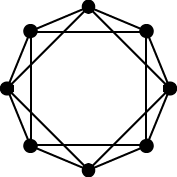
\includegraphics[width=4.073cm,height=4.073cm]{image/a2012Logique2eme-img057.png}
		\end{center}

	\end{Exercice}
	
	\begin{Exercice}{}
		Pour un graphe orienté donné par un tableau de listes d'adjacence, 
		écrire un algorithme qui détermine le n{\oe}ud de
		degré maximum. En cas d'ex-æquo, on retournera le n{\oe}ud 
		de plus petit indice.

	\end{Exercice}
	
	\begin{Exercice}{}
		Soit un graphe orienté donné par sa matrice d'adjacence. 
		Écrire un algorithme qui détermine le nombre de puits du
		graphe. \ Même question avec les sources.

	\end{Exercice}
	
	\begin{Exercice}{}
		Écrire l'algorithme qui calcule la matrice d'accessibilité 
		d'un graphe orienté par la formule de la somme des puissances
		de la matrice d'adjacence. 
		Quelle est la complexité de cet algorithme ? 
		Comparer avec la complexité de l'algorithme de Roy-Warshall.

	\end{Exercice}
	
	\begin{Exercice}{}
		Soit un graphe orienté donné par un tableau de listes (de la classe Liste). 
		Écrire l'algorithme qui permet de parcourir le graphe par contagion 
		à partir d'un n{\oe}ud de départ entré en paramètre. 

	\end{Exercice}
	
	\begin{Exercice}{}
		Soit un graphe orienté donné par un tableau de listes chainées. 
		Écrire l'algorithme qui donne sous la même forme le
		graphe issu de la matrice d'accessibilité du graphe de départ.
		
	\end{Exercice}
	
	\begin{Exercice}{}
		Soit un graphe dont les valeurs attachées aux n{\oe}uds 
		sont contenues dans un tableau valN{\oe}uds de $n$ entiers, 
		et soit $M$ sa matrice d'adjacence (tableau $n$ \textsf{x} $n$ 
		de booléens). Écrire un algorithme qui supprime de ce graphe 
		toutes les arêtes reliant deux n{\oe}uds de valeurs paires.
		
	\end{Exercice}
	
	\begin{Exercice}{}
		Dans un graphe orienté, une \textbf{racine} est un n{\oe}ud 
		à partir duquel on peut atteindre tous les autres n{\oe}uds.
		Écrire un module qui reçoit en paramètre la matrice d'adjacence 
		du graphe et un numéro de n{\oe}ud, et retourne un
		booléen indiquant si ce n{\oe}ud est une racine.

	\end{Exercice}
	
	\begin{Exercice}{}
		Un réseau de métro est composé de plusieurs lignes qui 
		peuvent se croiser en certaines stations. Les lignes sont
		implémentées dans un tableau \textbf{lignes} de listes~: 
		chaque élément du tableau est une liste chainée
		bidirectionnelle contenant les noms des stations dans 
		l'ordre de parcours d'une ligne donnée. Deux stations distinctes
		ont nécessairement des noms différents et une station 
		n'apparait qu'une seule fois pour chaque ligne.

		On demande d'implémenter une classe Réseau, en complétant le code 
		du constructeur et des 3 méthodes décrites ci-dessous~:

		\cadre{
			\begin{pseudo}
				\Class{Réseau}
					\Private 
						\RComment {à vous de donner les éléments privés}
					\Public 
						\ConstrSign{Réseau}{lignes~: tableau [1 à n] de ListeBi<chaine>}
						\MethodSign{getStations}{}{tableau [1 à m] de chaines}
						\LComment retourne le tableau des noms de toutes les stations du réseau
						\MethodSign{getAdjacence}{}{tableau [1 à m, 1 à m] de booléens}
						\LComment {retourne la matrice d'adjacence symétrique du graphe représentant le réseau.
						Chacune des stations est représentée par l'indice 
						que son nom a dans le tableau retourné par getStations( ).}
						\MethodSign{getDistance}{station1, station2~: chaines}{entier}
						\LComment {retourne la matrice des longueurs des chemins les plus courts 
						entre les différentes stations. Ici aussi chacune des stations est 
						représentée par l'indice que son nom a dans le tableau retourné par getStations( ).}
				\EndClass
			\end{pseudo}
		}
		
		\textbf{Remarque~:} on peut supposer que le réseau comporte moins de 
		500 stations et que le réseau est connexe.

	\end{Exercice}
	
	\begin{Exercice}{}
		Implémenter l'interface graphe dont les méthodes sont 
		décrites ci-dessous dans une classe (a) GrapheOrienté 
		(b) GrapheNonOrienté.
		
		\cadre{
			\begin{pseudo}
				\Interface{Graphe<T>}
					\MethodSign{getNbN{\oe}uds( )}{}{entier}
					\MethodSign{ajouteN{\oe}ud}{n{\oe}ud~: T}{}
					\MethodSign{retireN{\oe}ud}{indN{\oe}ud~: entier}{T}
					\MethodSign{setN{\oe}ud}{indN{\oe}ud~: entier, n{\oe}ud~: T}{}
					\MethodSign{getN{\oe}ud}{indN{\oe}ud~: entier}{T}
					\MethodSign{sontAdjacents}{indN{\oe}ud1~: entier, indN{\oe}ud2~: entier}{booléen}
					\MethodSign{getDistance}{indDepart~: entier, indArrivee~: entier}{entier}
					\MethodSign{getAccessibles}{indDepart~: entier, indArrivee~: entier}{booléen}
					\MethodSign{getSondage}{indDepart~: entier}{Liste<entier>}
					\LComment retourne la liste des n{\oe}uds dans l'ordre d'un parcours par sondage
					\MethodSign{getContagion}{indDepart~: entier}{Liste<entier>}
					\LComment retourne la liste des n{\oe}uds dans l'ordre d'un parcours par contagion
				\EndInterface
			\end{pseudo}
		}
		
	\end{Exercice}
	